\documentclass[10pt]{article}
\usepackage{icmlko}

\icmlmeta{IP 파운데이션 월드모델}{54}{내가 만든 결함을 내가 찾은 규칙이 잡았다}{같은 후보에 두 검정이 정반대 답을 냈다 --- 하나는 노트 53이 해롭다고 밝힌 조건을 검정 코드 안에서 재현하고 있었다}

\begin{document}

\twocolumn[
\icmlheader

\begin{abstract}
노트 53이 남긴 과제 --- 웹툰 매장 노출도를 강화하라 --- 부터 처리했다. 작가를
\emph{첫 한 명만} 매칭하고 있었는데 웹툰은 글작가와 그림작가가 따로인 경우가
절반이 넘는다(900건 중 454건). 전원 매칭에 이름 정규화까지 넣으니 이력 있는
레코드가 84건에서 135건으로, 라벨과의 상관이 $+$0.064에서 $+$0.099로 올랐다.
그런데 서른 셀 평균은 $+$0.3447에서 $+$0.3440으로 중립이다 --- 노트 53이 예측한
대로 현행 축이 이미 담고 있었다. 정확성 근거로만 유지했다. 그다음 노트 36에서
기각했던 고유 축 확장을 지금 눈금($\lambda=1.0$, 순위 기준)에서 다시 쟀다.
팝업은 여전히 $-$0.0167로 나쁘고 \textbf{게임만 $+$0.0066으로 좋다} --- 게임은
관측 축이 둘뿐이라 인자 공간이 사실상 회전만 하고 있었다. 짝지은 붓스트랩을
붙이니 \textbf{95\% 구간이 {[}$-$0.167, $-$0.027{]}로 완전히 음수}였다(P$=$0.000).
점추정과 정반대다. \textbf{검정 코드의 버그였다} --- 고유 축을 복원추출
\emph{뒤에} 붙여, 원본 순서의 축이 재추출된 행에 걸렸다. 노트 53이 ``레코드
대응을 깨면 축이 해롭다''고 밝힌 바로 그 조건을 내 검정 코드가 만들고 있었다.
순서를 고치니 \textbf{{[}$+$0.0014, $+$0.0110{]}, P$=$0.985로 채택}이다.
노트 53의 발견이 없었다면 ``게임 고유 축은 해롭다''를 그대로 기록했을 것이다.
정본에 통합해 현재 $\rho=+$0.3506이다.
\end{abstract}
]

\section{웹툰 매장 노출도부터}

노트 53이 짚었다 --- 웹툰 매장 노출도는 신호가 $+$0.087로 약한데 기여가
$-$0.0433으로 가장 크니 개선 여지도 가장 크다.

원인은 매칭이었다. 작가를 \emph{첫 한 명만} 보고 있었는데 웹툰은 글작가와
그림작가가 따로인 경우가 절반을 넘는다(900건 중 2인 이상이 454건).

\begin{table}[t]
\centering\tsize
\caption{웹툰 작가 매칭.}
\begin{tabular}{lrrr}
\toprule
& 이력 있는 것 & 건수 r & 최대 r \\
\midrule
첫 작가만 & 84/900 & $+$0.064 & $+$0.049 \\
\textbf{전원 $+$ 정규화} & \textbf{135/900} & \textbf{$+$0.099} & $+$0.095 \\
\bottomrule
\end{tabular}
\end{table}

이름 정규화도 함께 넣었다 --- 노트 52에서 아이돌 소속사의 `SM'과
`SM엔터테인먼트'가 따로 세어지는 것을 발견했으므로 같은 결함을 미리 막았다.

그런데 서른 셀 평균은 $+$0.3447에서 $+$0.3440으로 중립이다. \textbf{노트 53이
예측한 그대로다} --- 현행 축이 이미 담고 있어 개선이 안 옮겨진다. 성능 근거가
없으므로 \emph{정확성} 근거로만 유지했다. 같은 작가를 다르게 세는 것은 명백한
버그다.

\section{고유 축 확장을 다시 쟀다}

노트 36은 고유 축 확장을 기각했다. 그때는 $\lambda$가 겹침 유도였고 지표가
MAE 계열이었다. 지금 눈금에서 다시 쟀다.

\begin{figure}[t]
\centering

\includegraphics[width=\columnwidth]{figs/own.pdf}
\caption{도메인별 고유 축 확장.}
\end{figure}

\begin{table}[t]
\centering\tsize
\caption{고유 축을 더할 때. 현행 $\rho=+0.3440$.}
\begin{tabular}{lrr}
\toprule
도메인 & $\rho$ & $\Delta$ \\
\midrule
\textbf{게임} & \textbf{$+$0.3506} & \textbf{$+$0.0066} \\
도서 & $+$0.3423 & $-$0.0017 \\
아이돌 & $+$0.3386 & $-$0.0054 \\
팝업 & $+$0.3273 & $-$0.0167 \\
\bottomrule
\end{tabular}
\end{table}

게임만 좋아진다. 이유가 분명하다 --- 게임은 관측 축이 둘(타깃 폭, 굿즈 규모)뿐이라
성분 둘을 뽑으면 사실상 \emph{회전만} 한다. 넷을 더하면 처음으로 인자 공간이
정보를 압축한다. 나머지는 이미 넷에서 다섯 축을 관측하고 있어 더할 것이 적다.

\section{그런데 구간이 정반대였다}

\begin{figure}[t]
\centering
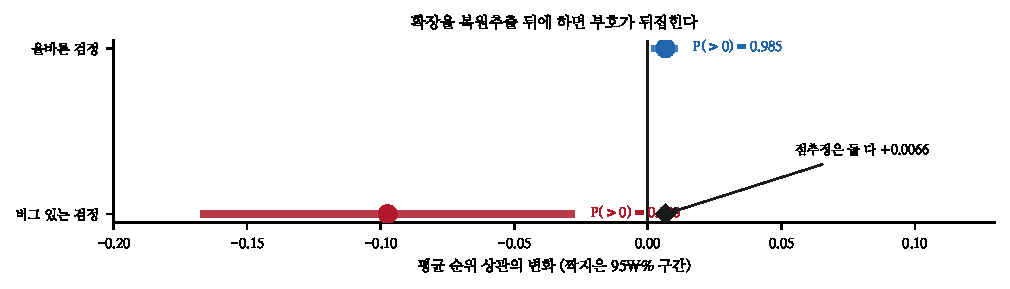
\includegraphics[width=\textwidth]{figs/bug.pdf}
\caption{같은 후보, 같은 점추정, 두 검정.}
\end{figure}

\begin{table}[t]
\centering\tsize
\caption{게임 고유 축의 짝지은 붓스트랩.}
\begin{tabular}{lrrr}
\toprule
검정 & 점추정 & 95\% 구간 & P($>$0) \\
\midrule
버그 있는 것 & $+$0.0066 & $[-0.167,\ -0.027]$ & 0.000 \\
\textbf{고친 것} & $+$0.0066 & $\mathbf{[+0.001,\ +0.011]}$ & \textbf{0.985} \\
\bottomrule
\end{tabular}
\end{table}

점추정이 같은데 구간이 정반대다.

\paragraph{버그의 정체}
복제마다 이렇게 했다 --- 도메인을 복원추출한 뒤 고유 축을 붙였다. 그런데 고유
축은 \emph{원본 순서}로 계산돼 있다. 복원추출은 크기를 보존하므로 길이는 맞고
오류도 안 난다. 다만 \textbf{어느 레코드의 값인지가 어긋난다.}

노트 53이 바로 그 조건을 검정했다 --- 실제 축 값을 그대로 두고 레코드 대응만
섞으면 $-$0.0352로 축을 끄는 것과 같아진다. \textbf{내 검정 코드가 그 해로운
조건을 복제마다 만들고 있었다.}

확장을 복원추출 \emph{앞}으로 옮기고 두 확장본을 같은 행 인덱스로 뽑게 고쳤다.

\claimx{검정 코드가 만드는 인공물은 결과의 부호까지 뒤집을 수 있다. 여기서는
노트 53이 독립적으로 밝혀 둔 성질 --- 레코드 대응이 깨지면 축이 해롭다 ---
덕분에 버그를 알아볼 수 있었다.}{이 진단이 맞다면 대응을 보존한 복제에서는
효과가 안정적이어야 한다. 200회 중 P$=$0.985이므로 그렇게 보이지만, 다른
씨앗에서 흔들리면 진단이 부족하다.}

\begin{quote}\fontsize{9.5}{11.5}\selectfont
노트 53은 축의 성질을 알아내려고 쓴 노트였는데, 그 결과가 한 노트 뒤에 \emph{내
도구의 결함}을 잡는 데 쓰였다. 시스템이 자기를 검사할 재료를 스스로 쌓는다.
\end{quote}

\section{정본에 통합했다}

게임 고유 축 넷(가격 · 연령 등급 · 최소 RAM · 기능 수)을 파이프라인에 넣었다.
슬롯 다섯 개 밖에 붙는 고유 축이므로 정렬에 참여하지 않고, 도메인마다 개수가
달라도 된다.

\begin{table}[t]
\centering\tsize
\caption{여섯 도메인 2,181건 · 서른 셀.}
\begin{tabular}{lrrrr}
\toprule
도메인 & n & 관측 축 & 자기 $\rho$ & 대상으로 \\
\midrule
아이돌 & 62 & 5 & $+$0.472 & $+$0.473 \\
웹툰 & 900 & 4 & $+$0.377 & $+$0.376 \\
팝업 & 75 & 5 & $+$0.368 & $+$0.452 \\
\textbf{게임} & 472 & \textbf{6} & $+$0.364 & \textbf{$+$0.377} \\
도서 & 242 & 4 & $+$0.202 & $+$0.225 \\
펀딩 & 400 & 4 & $+$0.190 & $+$0.199 \\
\midrule
\multicolumn{3}{l}{평균 $\rho$} & \multicolumn{2}{r}{\textbf{$+$0.3506}} \\
\bottomrule
\end{tabular}
\end{table}

게임이 대상일 때 $+$0.346에서 $+$0.377로 올랐다. 노트 36의 ``고유 축 확장은
소용없다''를 \textbf{게임에 한해 정정한다} --- 관측 축이 적은 도메인에서는
성립한다.

\section{한계}

\begin{itemize}[leftmargin=1.1em,itemsep=0.15em]
\item 버그를 고친 뒤의 구간이 $[+0.001,\ +0.011]$로 아래 끝이 0에 가깝다.
      씨앗 하나로만 쟀다.
\item 게임 고유 축 넷 중 연령 등급은 관측률이 낮아(54/482) 복제마다 결측 패턴이
      달라진다. 그 불안정이 구간에 얼마나 들어갔는지 모른다.
\item 같은 버그가 앞선 노트의 다른 검정에도 있었는지 전수 확인하지 않았다.
      고유 축을 쓴 검정은 노트 36과 이 노트뿐이라 범위는 좁다.
\item 웹툰 작가 매칭 개선을 성능 근거 없이 유지했다. 정확성이라는 근거는
      노트 48의 $\lambda$와 같은 종류이며, 그런 결정이 쌓이면 검정 없는 변경이
      늘어난다.
\item 게임 관측 축이 여섯이 되면서 다른 도메인과의 축 수 불균형이 커졌다.
      그 영향을 따로 보지 않았다.
\end{itemize}

\section{다음}

\begin{enumerate}[leftmargin=1.3em,itemsep=0.15em]
\item 웹툰 전체 완결작 3,073건 수집 --- 진행 중. 표본이 900에서 3,900이 되면
      노트 49의 ``큰 도메인을 늘리면 구간이 좁아지나''를 직접 검정한다.
\item 도서·펀딩에도 고유 축 후보를 찾는다. 둘 다 자기 $\rho$가 0.2 언저리로
      가장 낮다.
\item 구간을 여러 씨앗으로 다시 재 게임 고유 축을 굳힌다.
\item 검정 코드에 대응 보존을 강제하는 장치 --- 같은 버그를 세 번째로 만들지
      않도록.
\end{enumerate}

\vspace{0.6em}
\hrule height 0.3pt
\vspace{0.5em}
{\footnotesize
\textbf{참고문헌}\\[0.3em]
Efron, B., Tibshirani, R. J. (1993). \emph{An Introduction to the Bootstrap}.
Chapman \& Hall.\\[0.15em]
Meredith, W. (1993). Measurement invariance, factor analysis and factorial
invariance. \emph{Psychometrika}, 58(4), 525--543.\\[0.15em]
Bouthillier, X. et al. (2021). Accounting for variance in machine learning
benchmarks. \emph{MLSys}, 3, 747--769.\\[0.15em]
Gower, J. C., Dijksterhuis, G. B. (2004). \emph{Procrustes Problems}.
Oxford University Press.\\[0.15em]
Ben-David, S. et al. (2010). A theory of learning from different domains.
\emph{Machine Learning}, 79(1--2), 151--175.
}

\end{document}
